%-------------------------------------------------------------------------------
%	PACKAGES EN DOCUMENT CONFIGURATIE
%-------------------------------------------------------------------------------

\documentclass{uva-inf-article}
\usepackage[english]{babel}

\usepackage{tikz}
\usetikzlibrary{automata,positioning}

\usepackage{listings}

%-------------------------------------------------------------------------------
%	GEGEVENS VOOR IN DE TITEL
%-------------------------------------------------------------------------------

% Vul de naam van de opdracht in.
\assignment{Assignment 2}
% Vul het soort opdracht in.
\assignmenttype{Essay}
% Vul de titel van de eindopdracht in.
\title{Lexicographic Analysis}

% Vul de volledige namen van alle auteurs in.
\author{René Kok}
\uvanetid{13671146}

\author{Aram Mutlu}
\uvanetid{13574116}

% Vul eventueel ook de naam van de docent of vakcoordinator toe.
\docent{Dhr. dr. C.U. Grelck}
\course{Compiler Construction}
% Te vinden op onder andere Datanose.
\courseid{5062COMP6Y}

% Dit is de datum die op het document komt te staan. Standaard is dat vandaag.
\date{\today}

%-------------------------------------------------------------------------------
%	VOORPAGINA
%-------------------------------------------------------------------------------

\begin{document}
\maketitle

%-------------------------------------------------------------------------------
%	INHOUDSOPGAVE EN ABSTRACT
%-------------------------------------------------------------------------------

% Niet doen bij korte verslagen en rapporten
%\tableofcontents
%\begin{abstract}
%\lipsum[13]
%\end{abstract}

%-------------------------------------------------------------------------------
%	INTRODUCTIE
%-------------------------------------------------------------------------------

\section{Introduction}
\begin{flushleft}
\par This report provides information regarding the second assignment 
     "Lexicographic Analysis" of the course Compiler Construction given by Dhr. dr. C.U. Grelck. 
     The goal of this assignment is to create a Direct-coded Scanner of the regex "(ac$\mid$ab)*". To accomplish this we will pay particular attention to 
     Thompson’s Construction, Subset Construction, Hopcroft’s Algorithm and as last create a Direct-coded Scanner. In each section we will go deeper 
     in the steps taken to accomplish the goal of the assignment.

%-------------------------------------------------------------------------------
%	METHODE
%-------------------------------------------------------------------------------

\newpage
\section{Assignment}

\subsection{Thompson’s Construction}

    \par The first step in creating a direct code scanner is to create a 
         non-deterministic finite automaton (NFA) to recognize the regular expression
         "(ac$\mid$ab)*" using Thompson's Construction.

    \par It starts with defining an automaton that recognizes "ac" (see Figure ~\ref{fig:ThCoStep1}).

    \begin{figure}[h]
        \label{fig:ThCoStep1}
        \centering
        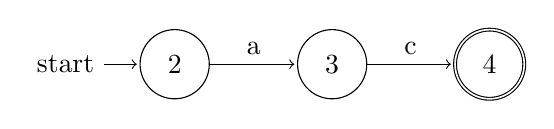
\begin{tikzpicture}[shorten >=1pt,node distance=2cm,on grid,auto] 
            \node[state, initial](2){2};
            \node[state, right=of 2](3){3};
            \node[state, accepting, right=of 3](4){4};
            \path[->] 
            (2) edge node {a} (3)
            (3) edge node {c} (4);
        \end{tikzpicture}
        \caption{Step 1 creating NFA for "ac" $\rightarrow$ (ac$\mid$ab)*}
    \end{figure}

    \par Then the automaton for recognizing "ab" is defined (see Figure ~\ref{fig:ThCoStep2}).

    \begin{figure}[h]
        \label{fig:ThCoStep2}
        \centering
        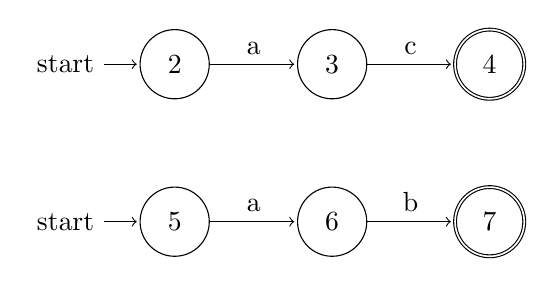
\begin{tikzpicture}[shorten >=1pt,node distance=2cm,on grid,auto]
            \node[state, initial](2){2};
            \node[state, right=of 2](3){3};
            \node[state, accepting, right=of 3](4){4};
            \node[state, initial, below=of 2](5){5};
            \node[state, right=of 5](6){6};
            \node[state, accepting, right=of 6](7){7};
            \path[->] 
            (2) edge node {a} (3)
            (3) edge node {c} (4) 
            (5) edge node {a} (6)
            (6) edge node {b} (7);
        \end{tikzpicture}
        \caption{Step 2 creating NFA for (ab) $\rightarrow$ (ac$\mid$ab)*}
    \end{figure}

    \par Because the regex expression matches either "ab" or "ab", the two automatons are linked by an alternation 
         (see Figure ~\ref{fig:ThCoStep3}).

    \begin{figure}[h]
        \label{fig:ThCoStep3}
        \centering
        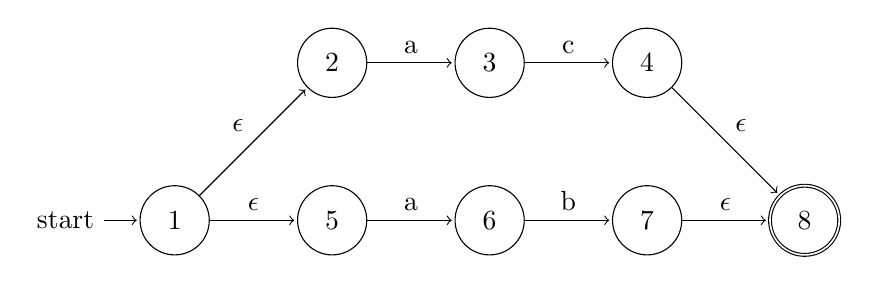
\begin{tikzpicture}[shorten >=1pt,node distance=2cm,on grid,auto] 
            \node[state, initial](1){1};
            \node[state, right=of 1](5){5};
            \node[state, above=of 5](2){2};
            \node[state, right=of 2](3){3};
            \node[state, right=of 3](4){4};
            \node[state, right=of 5](6){6};
            \node[state, right=of 6](7){7};
            \node[state, accepting, right=of 7](8){8};
            \path[->] 
            (1) edge node {$\epsilon$} (2)
                edge node {$\epsilon$} (5)
            (2) edge node {a} (3)
            (3) edge node {c} (4)
            (4) edge node {$\epsilon$} (8)
            (5) edge node {a} (6)
            (6) edge node {b} (7)
            (7) edge node {$\epsilon$} (8);
        \end{tikzpicture}
        \caption{Step 3 creating NFA for (ac$\mid$ab) $\rightarrow$ (ac$\mid$ab)*}
    \end{figure}
    
    \newpage
    \par As the last step of Thompson's construction, the alternations are added to the automaton, 
         creating the final automaton for the regex expression (see Figure ~\ref{fig:NFA}).

    \begin{figure}[h]
        \label{fig:NFA}
        \centering
        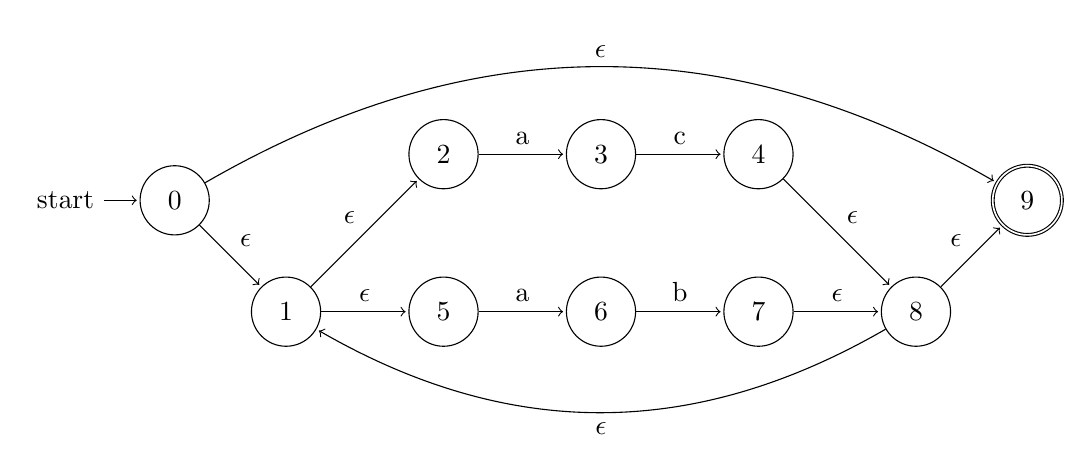
\begin{tikzpicture}[shorten >=1pt,node distance=2cm,on grid,auto] 
            \node[state, initial](0) {0};
            \node[state, below right=of 0](1){1};
            \node[state, right=of 1](5){5};
            \node[state, above=of 5](2){2};
            \node[state, right=of 2](3){3};
            \node[state, right=of 3](4){4};
            \node[state, right=of 5](6){6};
            \node[state, right=of 6](7){7};
            \node[state, right=of 7](8){8};
            \node[state, accepting, above right=of 8](9){9};
            \path[->] 
            (0) edge node {$\epsilon$} (1)
                edge [bend left] node {$\epsilon$} (9)
            (1) edge node {$\epsilon$} (2)
                edge node {$\epsilon$} (5)
            (2) edge node {a} (3)
            (3) edge node {c} (4)
            (4) edge node {$\epsilon$} (8)
            (5) edge node {a} (6)
            (6) edge node {b} (7)
            (7) edge node {$\epsilon$} (8)
            (8) edge node {$\epsilon$} (9)
                edge [bend left] node {$\epsilon$} (1);
        \end{tikzpicture}
        \caption{Final non-deterministic finite automaton for (ac$\mid$ab)*}
    \end{figure}

\newpage
\subsection{Subset Construction}
    \par Based on the NFA diagram (see Figure ~\ref{fig:NFA}), the following subset construction has been drawn up:
    \begin{table}[h!]
        \begin{center}
            \label{tab:table1}
            \begin{tabular}{l|c} % <-- Alignments: 1st column left, 2nd middle and 3rd right, with vertical lines in between
                \textbf{State} & \textbf{$\epsilon$-closures} \\
                \hline
                \{0\} & \{0, 1, 2, 5, 9\} \\
                \{1\} & \{1, 2, 5\} \\
                \{2\} & \{2\} \\
                \{3\} & \{3\} \\
                \{4\} & \{4, 8, 9, 1, 2, 5\} \\
                \{5\} & \{5\} \\
                \{6\} & \{6\} \\
                \{7\} & \{7, 8, 9, 1, 2, 5\} \\
                \{8\} & \{8, 9, 1, 2, 5\} \\
                \{9\} & \{9\} \\
            \end{tabular}
            \caption{Subset construction from NFA}
        \end{center}
    \end{table}

    \par With this subset construction the following DFA has been set up:

  \begin{figure}[h]
    \centering
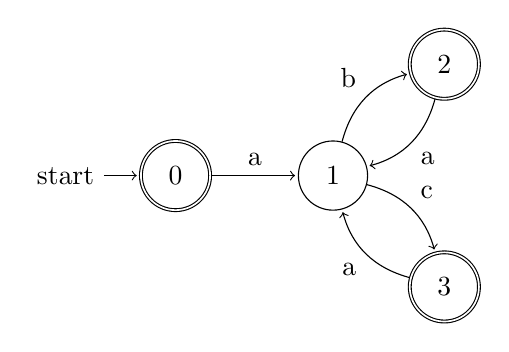
\begin{tikzpicture}[shorten >=1pt,node distance=2cm,on grid,auto] 
    \node[state, accepting, initial](0) {0};
    \node[state, right=of 0](1){1};
    \node[state, accepting, above right=of 1](2){2};
    \node[state, accepting, below right=of 1](3){3};
    \path[->] 
    (0) edge node {a} (1)
    (1) edge [bend left] node {b} (2)
        edge [bend left] node {c} (3)
    (2) edge [bend left] node {a} (1)
    (3) edge [bend left] node {a} (1);
\end{tikzpicture}
\caption{Deterministic finite automaton for (ac$\mid$ab)*}
\end{figure}
\subsection{Hopcroft’s Algorithm}
\begin{figure}[h]
    \centering
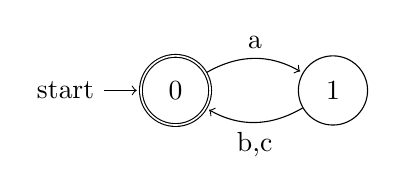
\begin{tikzpicture}[shorten >=1pt,node distance=2cm,on grid,auto] 
    \node[state, accepting, initial](0) {0};
    \node[state, right=of 0](1){1};
    \path[->] 
    (0) edge [bend left] node {a} (1)
    (1) edge [bend left] node {b,c} (0);
\end{tikzpicture}
\caption{Minimized deterministic finite automaton for (ac$\mid$ab)*}
\end{figure}
\newpage
\subsection{Direct-coded Scanner}
\lstinputlisting[basicstyle=\small, language=C]{scanner.c}
\end{flushleft}
\end{document}